\documentclass[a4paper,11pt]{article} 
\usepackage{mathpazo}
\usepackage{tikz}
\usetikzlibrary{shapes}
\oddsidemargin -0.54cm
\textwidth 17.0cm
\textheight 24cm
\topmargin -1.3cm
\parindent 0pt
\parskip 1ex
\pagestyle{empty}
\begin{document} 
\medskip\hrule\medskip
5 10 8 6 3 4 2 7 9 1000 are inserted

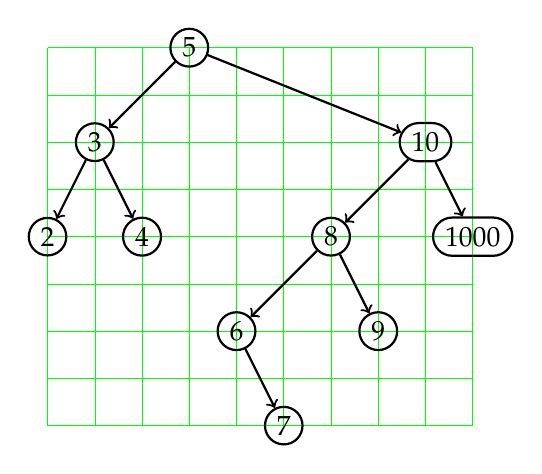
\begin{tikzpicture}[scale=0.600]
\draw [help lines, color=green] (1,-10) grid (10,-2); % creates help grid
\draw [thick] (10,-6) node[draw, rounded rectangle] (A) {1000};
\draw [thick] (8,-8) node[draw, rounded rectangle] (B) {9};
\draw [thick] (6,-10) node[draw, rounded rectangle] (C) {7};
\draw [thick] (5,-8) node[draw, rounded rectangle] (D) {6};
\draw [thick] (7,-6) node[draw, rounded rectangle] (E) {8};
\draw [thick] (9,-4) node[draw, rounded rectangle] (F) {10};
\draw [thick] (3,-6) node[draw, rounded rectangle] (A6) {4};
\draw [thick] (1,-6) node[draw, rounded rectangle] (CC6) {2};
\draw [thick] (2,-4) node[draw, rounded rectangle] (4_4) {3};
\draw [thick] (4,-2) node[draw, rounded rectangle] (abc) {5};
\draw [->, thick] (F) to (A);
\draw [->, thick] (E) to (B);
\draw [->, thick] (D) to (C);
\draw [->, thick] (E) to (D);
\draw [->, thick] (F) to (E);
\draw [->, thick] (abc) to (F);
\draw [->, thick] (4_4) to (A6);
\draw [->, thick] (4_4) to (CC6);
\draw [->, thick] (abc) to (4_4);
\end{tikzpicture}

\medskip\hrule\medskip
\end{document}
